\documentclass[14pt]{extbook}
\usepackage{multicol, enumerate, enumitem, hyperref, color, soul, setspace, parskip, fancyhdr} %General Packages
\usepackage{amssymb, amsthm, amsmath, bbm, latexsym, units, mathtools} %Math Packages
\everymath{\displaystyle} %All math in Display Style
% Packages with additional options
\usepackage[headsep=0.5cm,headheight=12pt, left=1 in,right= 1 in,top= 1 in,bottom= 1 in]{geometry}
\usepackage[usenames,dvipsnames]{xcolor}
\usepackage{dashrule}  % Package to use the command below to create lines between items
\newcommand{\litem}[1]{\item#1\hspace*{-1cm}\rule{\textwidth}{0.4pt}}
\pagestyle{fancy}
\lhead{Makeup Progress Quiz 1}
\chead{}
\rhead{Version A}
\lfoot{6018-3080}
\cfoot{}
\rfoot{Spring 2021}
\begin{document}

\begin{enumerate}
\litem{
Construct the lowest-degree polynomial given the zeros below. Then, choose the intervals that contain the coefficients of the polynomial in the form $ax^3+bx^2+cx+d$.\[ -3, \frac{-3}{4}, \text{ and } \frac{7}{3} \]\begin{enumerate}[label=\Alph*.]
\item \( a \in [12, 13], b \in [14, 21], c \in [-78, -75], \text{ and } d \in [61, 66] \)
\item \( a \in [12, 13], b \in [-57, -54], c \in [22, 39], \text{ and } d \in [61, 66] \)
\item \( a \in [12, 13], b \in [-23, -13], c \in [-78, -75], \text{ and } d \in [61, 66] \)
\item \( a \in [12, 13], b \in [14, 21], c \in [-78, -75], \text{ and } d \in [-63, -57] \)
\item \( a \in [12, 13], b \in [-78, -63], c \in [131, 136], \text{ and } d \in [-63, -57] \)

\end{enumerate} }
\litem{
Describe the end behavior of the polynomial below.\[ f(x) = 3(x - 9)^{5}(x + 9)^{6}(x - 3)^{3}(x + 3)^{4} \]\begin{enumerate}[label=\Alph*.]
\begin{multicols}{2}\item 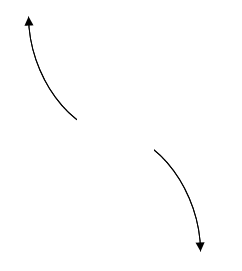
\includegraphics[width = 0.3\textwidth]{../Figures/polyEndBehaviorAA.png}\item 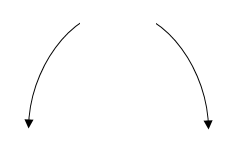
\includegraphics[width = 0.3\textwidth]{../Figures/polyEndBehaviorBA.png}\item 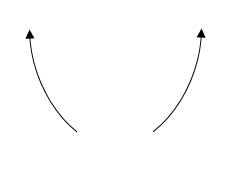
\includegraphics[width = 0.3\textwidth]{../Figures/polyEndBehaviorCA.png}\item 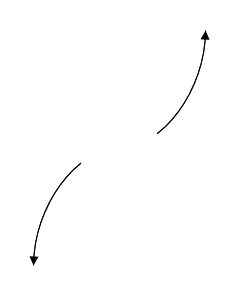
\includegraphics[width = 0.3\textwidth]{../Figures/polyEndBehaviorDA.png}\end{multicols}\item None of the above.
\end{enumerate} }
\litem{
Construct the lowest-degree polynomial given the zeros below. Then, choose the intervals that contain the coefficients of the polynomial in the form $x^3+bx^2+cx+d$.\[ -2 - 4 i \text{ and } 2 \]\begin{enumerate}[label=\Alph*.]
\item \( b \in [0.5, 1.3], c \in [-0.75, 0.06], \text{ and } d \in [-6.3, -3.5] \)
\item \( b \in [0.5, 1.3], c \in [1.85, 3.06], \text{ and } d \in [-10.4, -7.1] \)
\item \( b \in [-2.2, 0.7], c \in [11.7, 12.65], \text{ and } d \in [39.5, 42.6] \)
\item \( b \in [1.5, 2.9], c \in [11.7, 12.65], \text{ and } d \in [-41.8, -38.7] \)
\item \( \text{None of the above.} \)

\end{enumerate} }
\litem{
Construct the lowest-degree polynomial given the zeros below. Then, choose the intervals that contain the coefficients of the polynomial in the form $ax^3+bx^2+cx+d$.\[ \frac{7}{3}, \frac{-1}{4}, \text{ and } \frac{6}{5} \]\begin{enumerate}[label=\Alph*.]
\item \( a \in [57, 65], b \in [73, 89], c \in [-153, -150], \text{ and } d \in [-43, -39] \)
\item \( a \in [57, 65], b \in [-199, -195], c \in [108, 120], \text{ and } d \in [-43, -39] \)
\item \( a \in [57, 65], b \in [196, 200], c \in [108, 120], \text{ and } d \in [-43, -39] \)
\item \( a \in [57, 65], b \in [-199, -195], c \in [108, 120], \text{ and } d \in [33, 43] \)
\item \( a \in [57, 65], b \in [47, 60], c \in [-185, -182], \text{ and } d \in [33, 43] \)

\end{enumerate} }
\litem{
Construct the lowest-degree polynomial given the zeros below. Then, choose the intervals that contain the coefficients of the polynomial in the form $x^3+bx^2+cx+d$.\[ 5 - 4 i \text{ and } -1 \]\begin{enumerate}[label=\Alph*.]
\item \( b \in [-7, 7], c \in [-10, 4], \text{ and } d \in [-13, -4] \)
\item \( b \in [-9, -4], c \in [29, 36], \text{ and } d \in [37, 44] \)
\item \( b \in [4, 12], c \in [29, 36], \text{ and } d \in [-43, -39] \)
\item \( b \in [-7, 7], c \in [3, 13], \text{ and } d \in [0, 8] \)
\item \( \text{None of the above.} \)

\end{enumerate} }
\litem{
Which of the following equations \textit{could} be of the graph presented below?
\begin{center}
    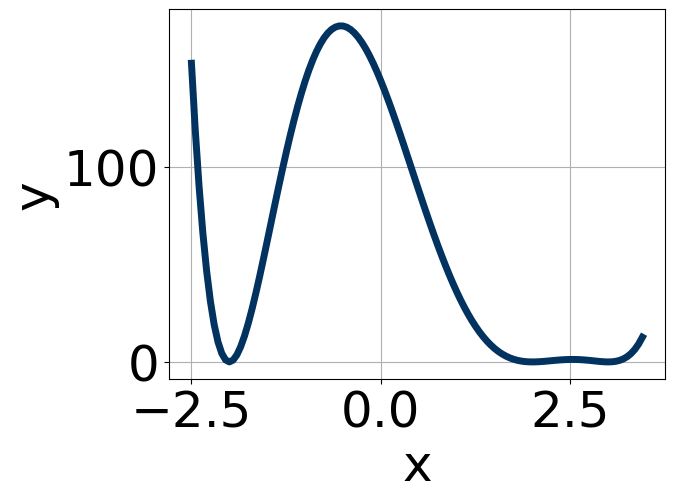
\includegraphics[width=0.5\textwidth]{../Figures/polyGraphToFunctionA.png}
\end{center}
\begin{enumerate}[label=\Alph*.]
\item \( 5(x - 2)^{6} (x + 2)^{11} (x - 3)^{7} \)
\item \( 17(x - 2)^{6} (x + 2)^{10} (x - 3)^{7} \)
\item \( -5(x - 2)^{4} (x + 2)^{10} (x - 3)^{4} \)
\item \( 16(x - 2)^{4} (x + 2)^{4} (x - 3)^{8} \)
\item \( -18(x - 2)^{8} (x + 2)^{4} (x - 3)^{7} \)

\end{enumerate} }
\litem{
Describe the zero behavior of the zero $x = -3$ of the polynomial below.\[ f(x) = -2(x - 3)^{2}(x + 3)^{3}(x - 4)^{4}(x + 4)^{7} \]\begin{enumerate}[label=\Alph*.]
\begin{multicols}{2}\item 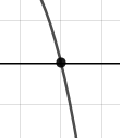
\includegraphics[width = 0.3\textwidth]{../Figures/polyZeroBehaviorCopyAA.png}\item 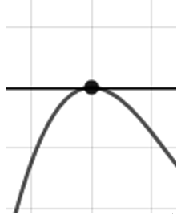
\includegraphics[width = 0.3\textwidth]{../Figures/polyZeroBehaviorCopyBA.png}\item 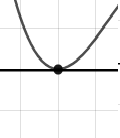
\includegraphics[width = 0.3\textwidth]{../Figures/polyZeroBehaviorCopyCA.png}\item 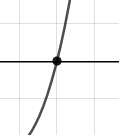
\includegraphics[width = 0.3\textwidth]{../Figures/polyZeroBehaviorCopyDA.png}\end{multicols}\item None of the above.
\end{enumerate} }
\litem{
Describe the end behavior of the polynomial below.\[ f(x) = 9(x - 7)^{4}(x + 7)^{5}(x + 6)^{3}(x - 6)^{4} \]\begin{enumerate}[label=\Alph*.]
\begin{multicols}{2}\item 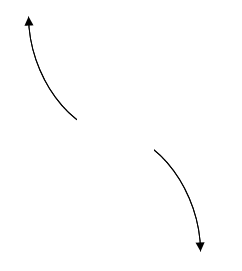
\includegraphics[width = 0.3\textwidth]{../Figures/polyEndBehaviorCopyAA.png}\item 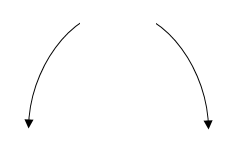
\includegraphics[width = 0.3\textwidth]{../Figures/polyEndBehaviorCopyBA.png}\item 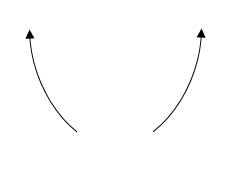
\includegraphics[width = 0.3\textwidth]{../Figures/polyEndBehaviorCopyCA.png}\item 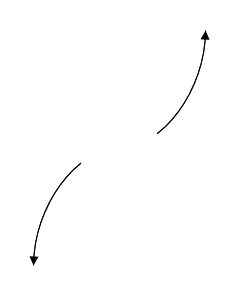
\includegraphics[width = 0.3\textwidth]{../Figures/polyEndBehaviorCopyDA.png}\end{multicols}\item None of the above.
\end{enumerate} }
\litem{
Which of the following equations \textit{could} be of the graph presented below?
\begin{center}
    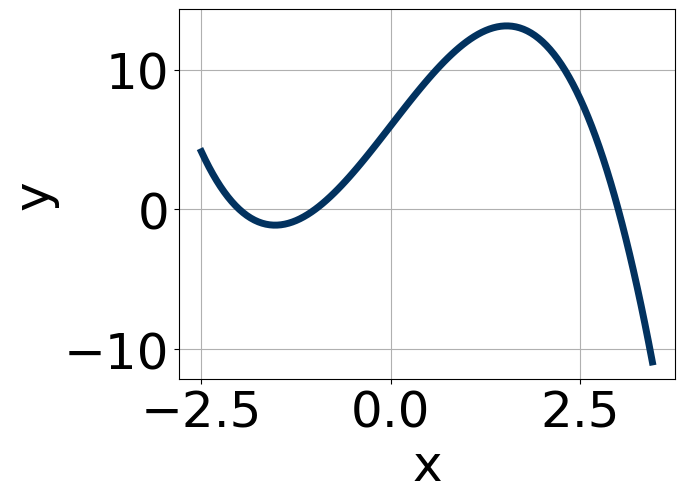
\includegraphics[width=0.5\textwidth]{../Figures/polyGraphToFunctionCopyA.png}
\end{center}
\begin{enumerate}[label=\Alph*.]
\item \( -3(x + 2)^{10} (x + 1)^{10} (x - 3)^{9} \)
\item \( 20(x + 2)^{7} (x + 1)^{11} (x - 3)^{7} \)
\item \( -2(x + 2)^{8} (x + 1)^{9} (x - 3)^{7} \)
\item \( -12(x + 2)^{11} (x + 1)^{5} (x - 3)^{9} \)
\item \( 10(x + 2)^{6} (x + 1)^{7} (x - 3)^{11} \)

\end{enumerate} }
\litem{
Describe the zero behavior of the zero $x = -3$ of the polynomial below.\[ f(x) = 3(x - 3)^{4}(x + 3)^{5}(x - 9)^{8}(x + 9)^{10} \]\begin{enumerate}[label=\Alph*.]
\begin{multicols}{2}\item 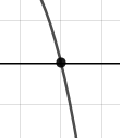
\includegraphics[width = 0.3\textwidth]{../Figures/polyZeroBehaviorAA.png}\item 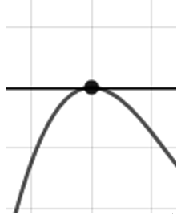
\includegraphics[width = 0.3\textwidth]{../Figures/polyZeroBehaviorBA.png}\item 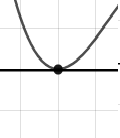
\includegraphics[width = 0.3\textwidth]{../Figures/polyZeroBehaviorCA.png}\item 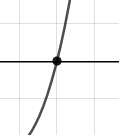
\includegraphics[width = 0.3\textwidth]{../Figures/polyZeroBehaviorDA.png}\end{multicols}\item None of the above.
\end{enumerate} }
\end{enumerate}

\end{document}